% !TEX encoding = UTF-8 Unicode
% !TEX root = HowToRobot.tex

%%%  This is the main driver file.   It is mostly a list of file includes.   Read through and edit as needed.

\documentclass[table]{book}


\usepackage[width=6.5in, height=9.0in, top=1.0in, papersize={8.5in,11in}]{geometry}
\usepackage[pdftex]{graphicx}
\DeclareGraphicsExtensions{.pdf,.png,.jpg}
%\usepackage{draftwatermark}
\usepackage{amsmath}
\usepackage{amsthm}
\usepackage{amssymb}
%\usepackage{txfonts}
\usepackage{textcomp}
%\usepackage{amsthm}
%\usepackage{array}
%\usepackage{datetime}
%\usepackage{anyfontsize}
\usepackage{cite}
\usepackage{enumitem}
\usepackage{t1enc}
\usepackage[section,subsection]{extraplaceins}   %%%  \FloatBarrier
\usepackage[all]{xy}
\usepackage{fancyhdr}
\usepackage{hyperref}
\usepackage{verbatim}
\usepackage{algorithm}
\usepackage{algorithmic}
\usepackage{makeidx}
\usepackage{multicol}
\usepackage{multirow}
\usepackage{color}
\usepackage{rotating}
\usepackage{wrapfig}
\usepackage{tikz}
\usetikzlibrary{shapes.geometric, arrows}
%\usepackage{tabularx}
\usepackage{xcolor}
%\usepackage{framed}
\usepackage{xspace}
\usepackage{listings}
\lstset{language=python,frame=ltrb,framesep=5pt,basicstyle=\normalsize,
 keywordstyle=\ttfamily\color{DarkRed},
%morecomment=[n][\textbf]{In\ [}{]\:},
%morecomment=[n][\textbf]{Out\ [}{]\:},
morecomment=[s][\color{blue}]{In\ [}{]\:},
morecomment=[s][\color{red}]{Out[}{]\:},
identifierstyle=\ttfamily\color{DarkBlue}\bfseries,
commentstyle=\color{OliveGreen},
stringstyle=\ttfamily,
showstringspaces=false,tabsize = 3}

\lstdefinelanguage{shell} {
commentstyle = \color{black},
keywordstyle = \color{black},
stringstyle = \color{black},
identifierstyle = \color{black},
morecomment=[s][\color{blue}]{In\ [}{]\:},
morecomment=[s][\color{red}]{Out[}{]\:},
 }

\newtheorem{thrm}{Theorem}
\newtheorem{lem}[thrm]{Lemma}
\newtheorem{cor}[thrm]{Corollary}
\newtheorem{rem}[thrm]{Remark}
\newtheorem{defn}[thrm]{Definition}
\newtheorem{exmpl}[thrm]{Example}

% this gives a little box for the end of a proof:
%
\def\endthrmbox{$\sqsubset \!\!\!\! \sqsupset$}

\newcommand{\dis}{\displaystyle}
 \def      \RR             {{\mathbb R}} 
        \def      \NN             {{\Bbb N}} 
        \def      \QQ             {{\Bbb Q}} 
        \def      \CC             {{\Bbb C}} 
        \def      \ZZ             {{\Bbb Z}} 
 
 
        \def       \a              {{\alpha}} 
        \def       \b              {{\beta}} 
        \def       \d              {{\delta}} 
        \def       \D              {{\Delta}} 
        \def         \e              {{\varepsilon}} 
        \def         \g              {{\gamma}} 
        \def         \G              {{\Gamma}} 
        \def       \l              {{\lambda}} 
        \def       \L              {{\Lambda}} 
        \def        \m               {{\mu}} 
        \def         \n              {{\nabla}} 
        \def       \var          {{\varphi}} 
        \def         \s              {{\sigma}} 
        \def       \Sig          {{\Sigma}} 
        \def       \Om          {{\Omega}} 
 
        \def       \t              {{\tau}} 
        \def         \th             {{\theta}} 
        \def       \O              {{\Omega}} 
        \def       \o              {{\omega}} 
        \def         \z              {{\zeta}} 
       \def        \P             {{\Phi}} 
       \def        \p             {{\phi}} 
        %Other macros 
 
        \def       \iy              {{\infty}} 
        \def         \pa             {{\partial}} 
        \def         \div           {{\rm div}} 
         \def       \na            {{\nabla}} 
 



\newcommand{\pythonlogo}{
\\[-2mm] \begin{picture}(0,0)
\put(-40,-40){\includegraphics[scale=0.25]{./Figures/pythonlogo.png}}
\end{picture}
}

\newcommand{\clogo}{
\\[-2mm] \begin{picture}(0,0)
\put(-30,-30){\includegraphics[scale=0.2]{./Figures/clogo.png}}
\end{picture}
}

\newcommand{\roslogo}{
\\[-2mm] 
\begin{picture}(0,0)
\put(-30,-30){\includegraphics[scale=0.2]{./Figures/roslogo.png}}
\end{picture}
}


\tikzstyle{master} = [rectangle, draw, text width=6em, text centered, minimum
height=3em]
\tikzstyle{node} = [rectangle, draw, text width=6em, text centered, rounded
corners, minimum height=3em]

\newtheorem{summary}{Summary:}
\newtheorem{example}{Example:}[section]

\definecolor{OliveGreen}{cmyk}{0.64,0,0.95,0.40}
\definecolor{DarkBlue}{cmyk}{0.76,0.76,0,0.20}
\definecolor{DarkRed}{cmyk}{0,1,1,0.45}


\def      \RR             {{\mathbb R}} 
\def      \DS            {\displaystyle} 

\setlength{\oddsidemargin}{0mm} 
\setlength{\evensidemargin}{0mm} 

%\SetWatermarkLightness{0.975}
%\SetWatermarkScale{6}
%\SetWatermarkText{\includegraphics{test.png}}

\pagestyle{fancy}
\renewcommand{\chaptermark}[1]{\markboth{#1}{}}
\renewcommand{\sectionmark}[1]{\markright{\thesection\ #1}}
\fancyhf{}
\fancyhead[LE,RO]{\bfseries\thepage}
\fancyhead[LO]{\bfseries\rightmark}
\fancyhead[RE]{\bfseries\leftmark}
\renewcommand{\headrulewidth}{0.5pt}
\renewcommand{\footrulewidth}{0pt}
\addtolength{\headheight}{0.5pt}
\setlength{\footskip}{0in}
\renewcommand{\footruleskip}{0pt}
\fancypagestyle{plain}{%
\fancyhead{}
\renewcommand{\headrulewidth}{0pt}
}


\definecolor{color02}{rgb}{0.18,0.35,0.59}
\definecolor{color03}{rgb}{0.44,0.59,0.82}
\definecolor{color06}{rgb}{0.35,0.35,0.35}


\definecolor{MSBlue}{rgb}{.204,.353,.541}
\definecolor{MSLightBlue}{rgb}{.31,.506,.741}
\definecolor{MSBlue1}{rgb}{0.18,0.35,0.59}
\definecolor{MSBlue2}{rgb}{0.44,0.59,0.82}
\definecolor{MSBlue3}{rgb}{0.35,0.35,0.35}

\usepackage{titlesec}
\titleformat{\chapter}[display]
%{\normalfont\bfseries\color{MSBlue1}}    %\normalfont\bfseries\filcenter}
{\normalfont\bfseries}    %\normalfont\bfseries\filcenter}
{\LARGE\thechapter}
{1ex}
{\titlerule[2pt]
\vspace{2ex}%
\LARGE}
[\vspace{1ex}%
{\titlerule[2pt]}]



\date{\today}

 % This sets the format.

% Add your title page contents here 
\title{{ \rule{\linewidth}{0.5mm}}\\[2mm] {\huge \bfseries  How To Build a ROS Robot }\\[-1mm] {\rule{\linewidth}{0.5mm}} \\  \vfill
{\LARGE \bfseries  SDSMT Robotics Team }\vfill}
\author{Ian Carlson }
\date{\today}



\begin{document}

\maketitle

\frontmatter

\addcontentsline{toc}{chapter}{Title}
\maketitle
\tableofcontents
\addcontentsline{toc}{chapter}{Contents}
\listoffigures
\addcontentsline{toc}{chapter}{List of Figures}
%\listoftables
%\addcontentsline{toc}{chapter}{List of Tables}
%\listofalgorithms
%\addcontentsline{toc}{chapter}{List of Algorithms}
 
 
\mainmatter
% !TEX root = HowToRobot.tex

\chapter{Introduction}
\label{chap:intro}

\section{Purpose}
Building a sophisticated robot can be a complex and potentially daunting task. While a single afternoon can be sufficient to strap a few servos and an arduino to a chassis, doing anything interesting required an investment of both time and resources. As the cost of a robot increases, it becomes more important to have a solid plan to follow. This document attempts to outline the major phases of robotics development, as well as providing the basic information required to build a basic robot featuring ROS. It should be noted that this document is entirely a product of my own experiences - mostly the failures - during my time on the Robotics team, in the hope that others will not repeat them. That being said, this document is neither expected to be entirely complete nor perfectly accurate. It is a certain truth that failure is a better teacher than success, but experience is the best teacher of all - preferably someone else's.

The major sections are as follows:
\begin{itemize}
\item{Mechanical Design - Basic mobile robot kinematics and design principles.}
\item{Electrical Design - How not start your robot on fire. Probably.}
\item{Setting Up The Odroid - How to go from a fresh Odroid to one running Fedora 22 and ROS}
\item{ROS Architecture - The basic design for a remote controlled robot in ROS}
\end{itemize} 

This guide should be delivered alongside its companion document - Robot Paper Template - and potentially the example I created using that template - Mecanum and SMP Design Document. All of the code referenced in this document is available on the SDSMT Robotics Team GitHub pages - SMD-ROS-DEVEL and SMD-ROBOTICS. \\
% !TEX root = HowToRobot.tex

\chapter{Mechanical Design}
\label{chap:MechDes}

\section{Design Considerations}
One hugely important aspect of your robot design is ensuring it is mechanically capable of fulfilling requirements - and making sure it doesn't collapse under its own weight. No amount of sophisticated code, nor the most powerful computer in the world, can force your robot to function if the chassis is compromised. It is tempting - we fell in to this trap several times during my time on the Robotics Team - to want to design your perfect robot from the ground up. Don't. If this is your first robot, or even second or third, take my word for it and just buy a chassis.

Seriously.

Mechanical design is time-consuming and, unless you have several skilled mechanical designers around, likely going to be difficult. On the Mines campus, it has become increasingly difficult to do any real fabrication, thanks in part to the increasingly strict attention to safety, and the CAT lab's understandable desire to cut down on machining costs.\\

Going for it anyway? Good for you, however, keep a few things in mind:

First, keep it simple. Complex designs are more expensive, have tighter tolerances, take a great deal longer to design and fabricate, and - most importantly - have more ways to fail. The best design in the world is useless if it never makes it off paper.

Second, keep moving parts to a minimum. This is similar to point one, but it's important enough to say twice. Every moving part means you need to deal with routing power i.e. keeping cables from getting tangled. Every moving piece also generally adds weight, cost, and complexity.

Third, if the words "we'll attach this here somehow" are ever uttered, take a closer look. We like to think in the CSC department that Mechanical Engineering is just hitting things with hammers and turning wrenches, but building real things is actually very difficult. Every piece of your robot has to be attached somehow - avoid glue - and that's not something that just sorts itself out once you have all the pieces.

Fourth - No, hot glue is not a good idea. Trust me. Been there. It's not. Epoxy can work, but it's no substitute for bolts.

Fifth - 3M velcro tape is better, but still not good, and is only appropriate for an indoor non-competition research vehicle where frequent reconfiguration is expected. See the SMP and Mecanum chassis for examples. It doesn't hold up under vibration as well as you would think. It holds great against normal stress, but not terribly well against sheer stress, and not at all against twisting stress.

Sixth, iterate. Don't expect your first build to be perfect. In all honesty, it probably won't even work. You forgot something or overlooked something or assumed something that isn't right. I promise. Give me a call before you start designing, and I will bet you \$100. Expect your design to fail, and get something built as early as possible. A failed design isn't the end of the world unless it's the day of competition. More than one of our designs failed because we were half-way into the spring semester before we got anything built, and there was no time to try again.

Seventh, failure is good. You learn a whole lot from mistakes. Don't be afraid to try something just because it might not work. It \textit{definitely} won't work the first time anyway.

\section{Requirements}

What does your robot need to do? Agile development is great for software, and there are some applications that can be adapted to hardware, but you really need to know what you're getting into before you start buying or building things. I can't possibly predict every possible requirement, but here are a few important ones I have come across before.

How does the robot need to move? Whether mobile or fixed, your robot likely needs to actuate within its workspace, and this will be one of the main factors in the mechanical design.This will be addressed further in section \ref{section:kinematicModels}.

How fast does the robot need to be? If your robot doesn't need to be very fast, you can reduce power requirements, use smaller and/or cheaper motors, and you don't have to worry as much about vibrations. If the robot needs to be fast, the inverse is true.

How strong does the robot need to be? If the robot only needs to drive from A to B on a card table carrying a few paperclips, an Arduino taped to a few continuous rotation servos and some cardboard will probably do the trick. If you need to carry a cinderblock around an outdoor obstacle course, you need a robust frame, bigger motors, bigger batteries, and space to put it all.

How durable does the robot need to be? This one is pretty self-explanatory. However, keep in mind that as soon as you have a working RC robot, people will want to play with it. They will crash it. Hard. Once the robot is driving autonomously, it will crash itself. Often \textit{and} hard. Make sure all potential contact surfaces on the robot can survive impact at maximum speed with something sharp and/or hard.

Does it need to be waterproof or water-resistant? Some competitions - like the Sparkfun AVC - are outdoors. Given Murphy's law, this means it will probably rain. Plan early about ways to keep water out and the magic smoke in. Never put holes in the top, and consider rubber grommets or seals around connectors and cabling. Also consider having angled non-porous surfaces on the top of the robot to deflect water such that it will drip harmlessly away from the electronics.

Does it need to be heat-tolerant? This, unfortunately, is in direct conflict with being waterproof, because you need to put holes in the robot for air circulation. We never came up with a perfect solution that handles both. Assume your CPU, GPU (if you have one), motor controller, and motors will attempt to melt anything in contact with them as soon as you close the case. Make sure you have proper heat-sinking and, if possible, forced air-flow over those heat-sinks. Also make sure the air has a way to escape. If operating outdoors, make sure you have filtered air intake.

Finally, what does it need to do? Claws, grippers, baskets, sensors, and payloads all need secure mounting. Make sure you include some sort of mounting bracket for whatever tools your robot will need to complete its job.

\section{Kinematic Models}\label{section:kinematicModels}

Now that you know what your robot needs to do, it's time to actually start designing something. For a mobile robot, kinematics are everything. There are a few common kinematic models that I want to cover in some detail.

Each kinematic model has different advantages and disadvantages, so it is important to consider how your robot needs to be able to move before selecting one.

\subsection{Differential Drive}

The simplest and most common drive system for a mobile robot is differential drive. This involves a fixed axle with two independently driven motors at the ends. A picture is worth a thousand words, so check out Figure \ref{fig:diffdrive}, borrowed from the nice people at www.robotplatform.com.

\begin{figure}[h]
\centering
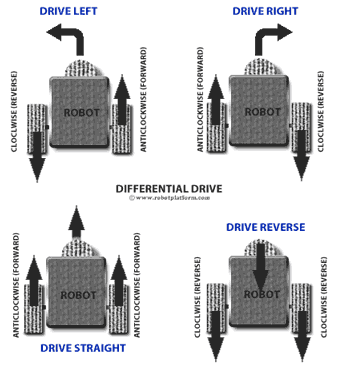
\includegraphics[width=0.6\textwidth]{Differential_Drive.png}
\caption{Differential Drive}
\label{fig:diffdrive}
\end{figure}

Differential Drive is very simple because it only requires two powered wheels. In the image, the front wheel is a caster wheel, or a skid-pad, and is only present to keep the robot upright.

One major advantage of the differential drive paradigm is the ability to turn in place by spinning one wheel forward, and one back. However, because of the skid-pad or caster wheel, differential drive is typically only used in low-speed applications. The extra drag and wobbling of an uncontrolled wheel could cause vibrations or instability at high speeds.

%I won't go into the derivation of the kinematic model, but I will present it here so you can use it for reference. There %are two kinematic models of interest, the forward kinematic model and the inverse.

%The reverse kinematic model tells you how the robot will move given a set of wheel velocities, and is shown in Equation %\ref{eqn:diffdriveforward}.

%TODO: Add kinematics?

\subsection{Ackermann Drive}

Ackermann drive is a common choice for high speed robots because it provides better stability and less drag than the differential drive. It is also the same steering system that most cars use. However, an Ackermann steered vehicle cannot turn in place.

An Ackermann drive vehicle must have two front wheels which can be turned, and two fixed rear wheels. It is common to have powered rear wheels since the pivoting front wheels adds additional complexity when attempting to mount motors, but powered front wheels are not unheard of. See Figure \ref{fig:ackermann}.

\begin{figure}[h]
\centering
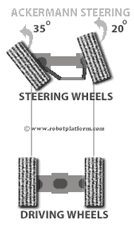
\includegraphics[width=0.25\textwidth]{Ackermann_Drive2.png}
\caption{Ackermann Drive}
\label{fig:ackermann}
\end{figure}

There is one additional complication to consider when attempting to build your own Ackermann Drive system. When an Ackermann vehicle turns, each wheel is essentially drawing out the circumference of a circle. To take that thought a step further, both steering wheels will be drawing out circles, but of slightly different radii - the difference being the center to center distance from wheel to wheel. Therefore, to avoid wheel slip while drawing two circles of different sizes, each wheel must be at a slightly different angle. The difference changes depending on how sharp of a turn is desired. Obviously designing a mechanical system to automatically handle this would be complex, and writing code to handle turning each wheel individually would be non-trivial at best. I will once again recommend buying a professionally made drive system over building one unless you have a really good reason not to.

%TODO: Add kinematics?

\subsection{Skid Steer}
\label{sec:skidsteer}
Skid Steer A.K.A. Tank Drive, is another common form of locomotion. It's similar two having two differential drive systems mounted with a rigid bar between them. See Figure \ref{fig:skid_steer_drive} for an example of how Skid Steer drives. Each side, regardless of how many wheels it has, is unified, meaning that all wheels on the left drive at the same time and speed, as do all the wheels on the right. Tank drive is arguably better for an outdoor robot because it is much harder to end up high-centered when all of your wheels are powered. This also gives you more traction. However, to do anything other than drive straight forward or backward, some of the wheels have to slip. The largest disadvantage to Skid Steer is that any sort of wheel speed or encoder based odometry becomes very unreliable.

\begin{figure}[h]
\centering
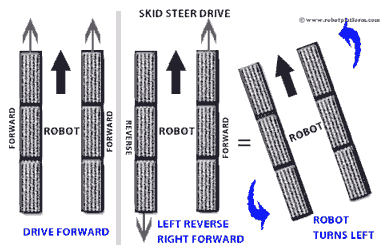
\includegraphics[scale=0.7]{skid_steer_drive.png}
\caption{Skid Steer}
\label{fig:skid_steer_drive}
\end{figure} 

However, if you have some other means of localization, like the LIDAR on the SMP robots, or the ASUS RGBD sensor, this becomes less of a problem. You end up with less drag than traditional differential drive and potentially more power because each wheel may (but doesn't have to) have its own motor. In addition, this design is much simpler to implement than Ackermann Steering or Omni-Drive, which will be discussed next. For these reasons, the SMP robots use Skid Steer. See the SMP in Figure \ref{fig:smprobot}.

\begin{figure}[h]
\centering
\includegraphics[width=.7\textwidth]{smprobot.png}
\caption{SMP Robot}
\label{fig:smprobot}
\end{figure} 

\subsection{Omni-Driv}

An Omni-Drive robot is one that can move in any direction. There are several ways to construct an Omni-Drive robot, but I will focus on a four wheeled robot with fixed wheels in "traditional" positions. The Mecanum robot shown in Figure \ref{fig:mecanumrobot} - named so for the style of wheels - is one such robot.

\begin{figure}[h]
\centering
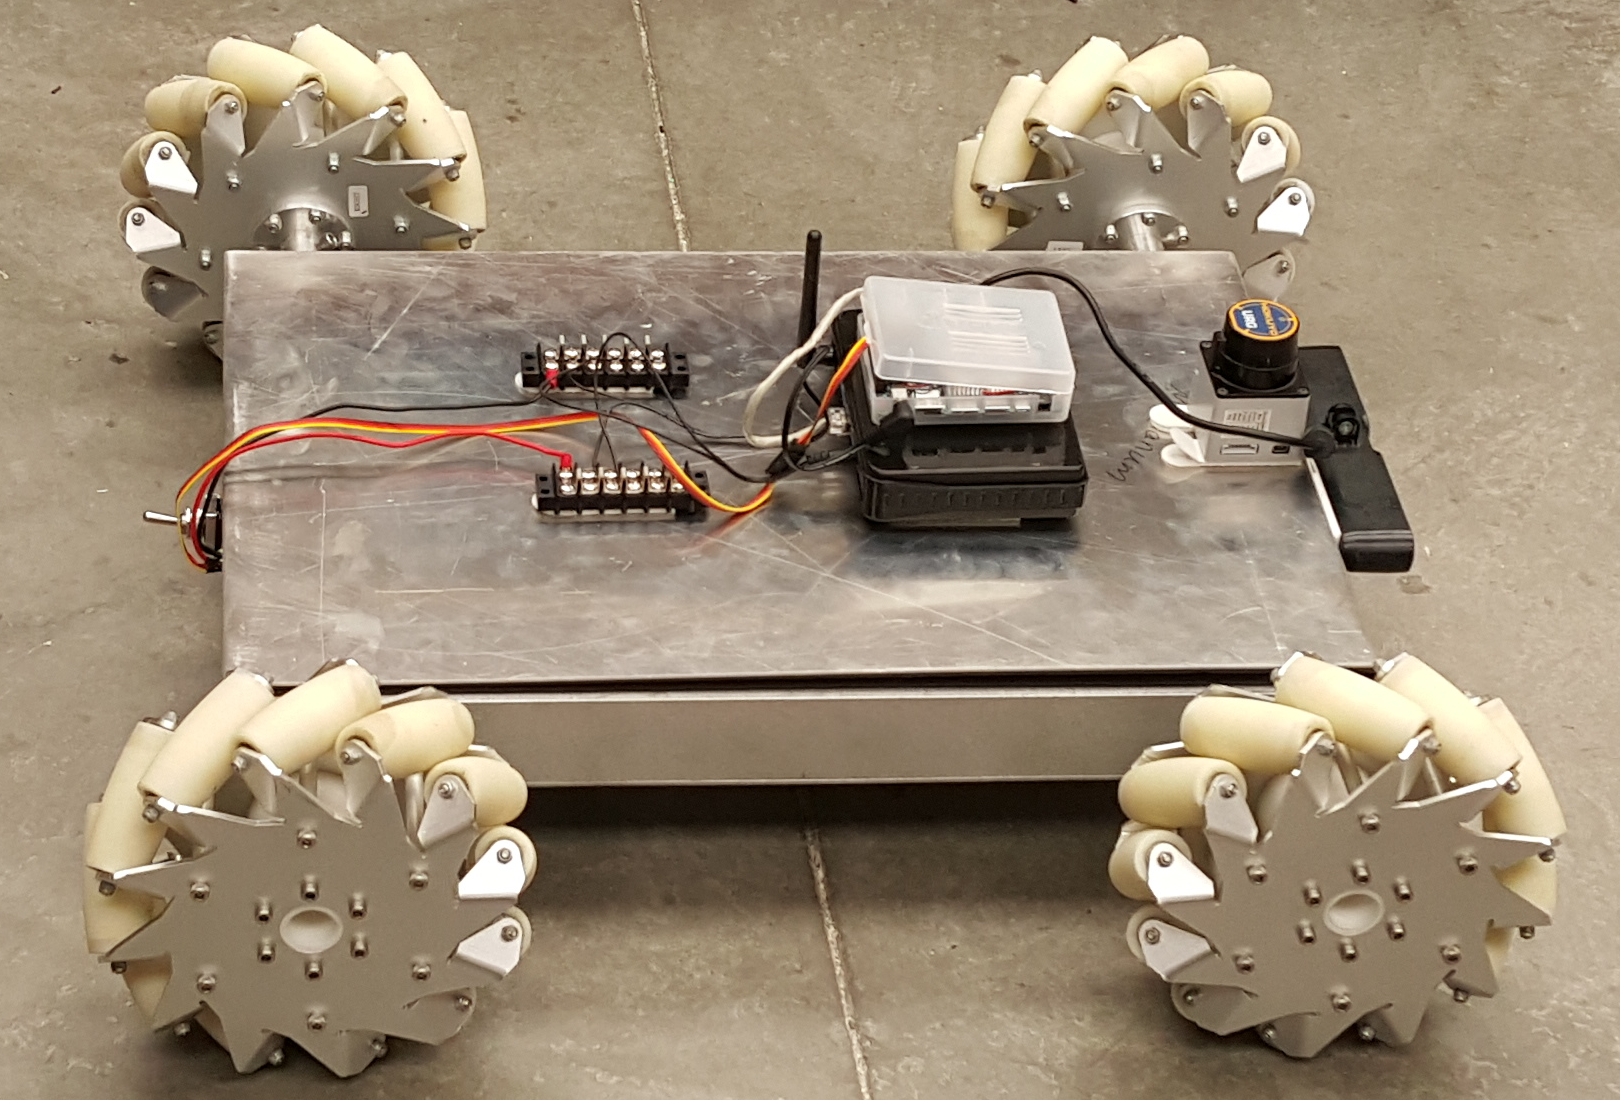
\includegraphics[width=.65\textwidth]{mecanumrobot.png}
\caption{Mecanum Robot}
\label{fig:mecanumrobot}
\end{figure} 

%\begin{figure}
%\centering
%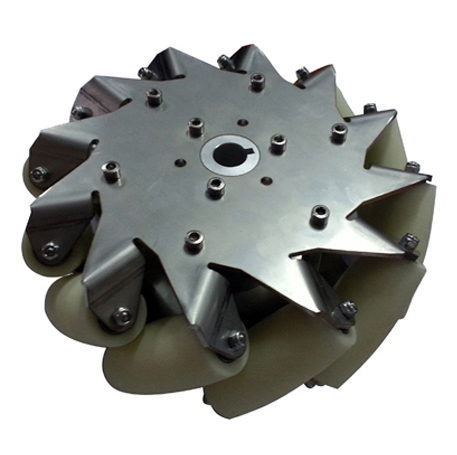
\includegraphics[width=0.45\textwidth]{mecanumwheels.png}
%\caption{Mecanum Wheel}
%\label{fig:mecanumwheels}
%\end{figure} 

Omni-Drive kinematics are complex, but I will attempt a brief summary. The rollers on this style of mecanum wheel are mounted at 45 degrees. The means that of any amount of force applied to rotating a wheel, only approximately half will be exerted along the line parallel with the direction of travel. The other half will be exerted along the perpendicular axis. The wheels are not mounted symmetrically, however. All wheels are mounted such that, if all wheels turn forward, the perpendicular forces will cancel, allowing the robot to move forward. By operating the wheels in opposing pairs, a force in any direction can be generated, allowing the robot to translate and rotate in any direction freely. Figures \ref{fig:mecanumlocomotion} shows examples of the motion generated by various combinations of wheel speeds. This is very useful for a robot, because it means there aren't any constraints that have to be considered when attempting to operate the robot autonomously. If you want to move in a certain way, you can, no questions asked.


\begin{figure}
\centering
\begin{subfigure}{.5\textwidth}
  \centering
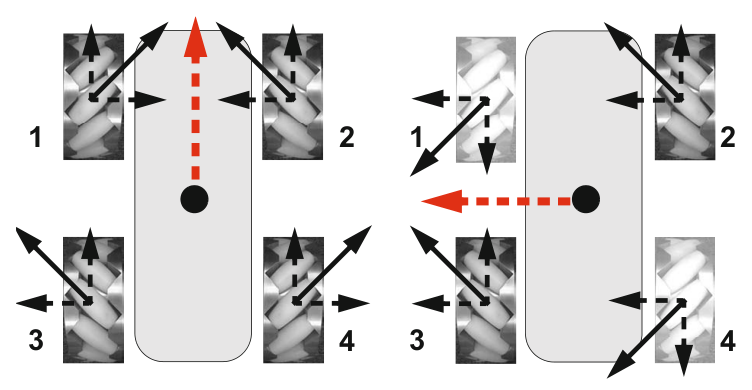
\includegraphics[width=\textwidth]{swedish_vector2.png}
  \caption{Translation}
  \label{fig:sub1}
\end{subfigure}%
\begin{subfigure}{.5\textwidth}
  \centering
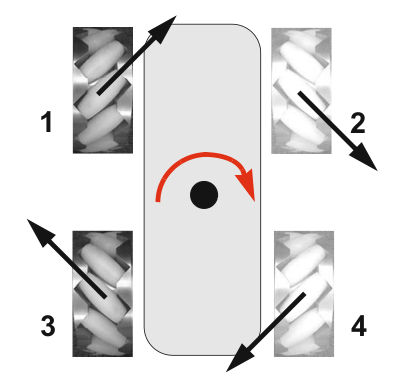
\includegraphics[width=.5\textwidth]{swedish_vector3.png}
  \caption{Rotation}
  \label{fig:sub2}
\end{subfigure}
\caption{Mecanum Locomotion}
\label{fig:mecanumlocomotion}
\end{figure}

While the actual mathematics for driving an Omni-Drive robot are relatively complex, the concept is simple. Just calculate the translation you want to preform, then the rotation, and add them. In this case, the total is just the sum of the parts. Special care should be taken, however. Attempting to both drive forward and turn at full speed works fine mathematically, but once you command a wheel to drive faster than its top speed, the robot will begin to behave erratically as the forces will no longer properly cancel.




























% !TEX root = HowToRobot.tex

\chapter{Electrical Design}
\label{chap:ElecDes}

\section{Design Considerations}
The most important aspect of your robot is ensuring that it is electrically capable of fulfilling requirements - and making sure it doesn't light itself on fire or electrocute anyone. The best mechanical design in the world is useless if there's nothing to supply power to the wheels, and your computer is just a hunk of plastic and metal if it doesn't get the right amount of power. While electrical design for a robot is not very complicated (unless you want it to be), it does require some fundamental knowledge.

\subsection{The Basics}
We'll start off easy. I'm going to restrict the discussion here to (relatively) low voltage DC circuits. Within that domain, there are three very important terms. Voltage, measured in Volts (V), Current, measured in Amperes "Amps" (A), and Resistance, measured in Ohms $\Omega$. A very smart German dude by the name of Georg Ohm came up with probably the most important (for us at least) law in all of electronics back in 1827, and published it in his book Die \textit{galvanische Kette, mathematisch bearbeitet}. (Translated to English, that's \textit{The Galvanic Circuit Investigated Mathematically}). The book is available online, but I wouldn't recommend it unless you're in for some heavy reading. It was written in the early 1800s after all. The important part - the law we care about here - is called Ohm's law and is shown in Equation \ref{eqn:ohmslaw}.

\begin{equation}
V = IR
\label{eqn:ohmslaw}
\end{equation}

That's it. That's all there is to it. Voltage (V) equals Current (I) times Resistance(R). This law has the interesting property that, unlike everything else we do in Electrical Engineering, it almost always holds true. So, if something isn't behaving the way you think it should, refer to this law.

Ok, so now we have the fundamental law of the universe, but so what? What are all these funky terms? Let's talk more about that. Sparkfun also has a pretty excellent page explaining this, so if my explanation doesn't work out for you, just search for \textit{Sparkfun Voltage, Current, Resistance, and Ohm's Law}.

\subsection{Voltage}
Voltage behaves very much like water pressure in a pipe. With water, pressure - or more accurately, pressure differential - is what causes water to flow. However, just because there is pressure doesn't mean the water actually flows. It's just a measure of how much the water \textit{wants} to flow. For example, consider a completely full, sealed container of water. Now shrink the volume of the container by half without letting any water out. Some laws that I vaguely remember from chemistry say that the pressure has to increase. (Or temperature, but likely it will be some of both). Now there's more pressure, but the container is still sealed with no route for the water to escape, so there's no flow.

Voltage behaves almost exactly the same. Except instead of water, we have a high density of electrons. Because they are negatively charged, and like charges repel one another, electrons like to spread out as much as they can to reach the minimum energy configuration. Sort of like when you drop a glass of water on the floor, and the water spreads out to get as low to the ground as possible - thereby reducing it's gravitational potential energy and reaching a minimal energy state. So, compressing a lot of electrons in to a small space creates this electrical pressure - voltage, or electromotive force for people who like words with many syllables.

The common source of voltage differentials in mobile robotics are batteries or DC power supplies.

\subsection{Current}

If voltage is pressure, than current is the amount of flow. If there is a pressure differential, and a route for water to escape, then flow happens in a pipe. This flow continues until the pressure differential is balanced out. Batteries work the same way. (By the way, think of power supplies as infinite batteries.) A fully charged battery has some voltage, and if there is a path from the negative terminal to the positive terminal, electrons will flow along that path. As the electrons flow from negative to positive and thereby "spread out" to the minimal energy state, the battery voltage will decrease. This flow is current.

\subsection{Resistance}

Resistance is not a property of the electricity itself, but a property of the material it flows through. The easy analogy is to think of the resistance as the size of the pipe. A narrower pipe allows less water to flow through. Likewise, a material with higher resistances "resists" the flow of electrons more strongly. In low power DC applications, you can generally assume that wires have a resistance of 0.

Often, we will use components called "Resistors" to purposefully introduce current in a circuit. This is particularly useful when we have components like LEDs (light-emitting diodes) which can only handle so much current. We'll have an example circuit a little later demonstrating how to choose the right resistor for an LED.

There is one more thing you need to know about resistors before we move on. What happens if you have more than one? There are two ways to hook up multiple resistors. You can put them in parallel or in series. In Figure \ref{fig:seriesresistors} - from wikipedia, which covers this subject in great depth- there are N resistors hooked up in series. This case is very easy. The value of the resistors just adds up, so you can pretend like you have one big resistors with a value that is the sum of all the resistors in series. Because I like math, the oh-so-difficult math for this is shown in Equation \ref{eqn:seriesresistors}.

\begin{equation}
R = R_1 + R_2 + \cdots + R_n
\label{eqn:seriesresistors}
\end{equation}

\begin{figure}[h]
\centering
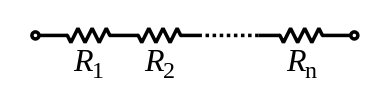
\includegraphics[scale=0.75]{seriesresistors.png}
\label{fig:seriesresistors}
\caption{Resistors In Series}
\end{figure}

The other way to hook up resistors is in parallel. This one is a little more complicated. An example is shown in Figure \ref{fig:parallelresistors}.

\begin{figure}[h]
\centering
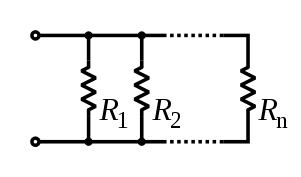
\includegraphics[scale=0.75]{parallelresistors.png}
\label{fig:parallelresistors}
\caption{Resistors In Parallel}
\end{figure}

\subsubsection{Putting It All Together}

Example time! First, look at the picture in Figure \ref{fig:voltagedivider}. In that example, there are multiple paths for the electricity to follow. Meditating on Ohm's law for a while will eventually lead you to the mathematical reason behind this, but for now just take my word for it: the electricity divides itself up among the possible paths inversely proportional to the resistance of each path. Ohm's law requires this, and it's actually convenient for us because it generates the least possible waste heat - but that's an advanced topic I won't cover here. Let's attach some real numbers to this example. Consider a circuit with a 10V voltage source and 2 resistors in parallel, one with 5$\Omega$ and one with 10$\Omega$. This example circuit is shown in Figure \ref{fig:parallelresistorsexample}. Reducing the two resistors with Equations \ref{eqn:parallelresistors}, gives the circuit showin in Figure \ref{fig:parallelresistorsexamplemerged}.


\begin{figure}
\centering
\begin{minipage}{.5\textwidth}
\centering
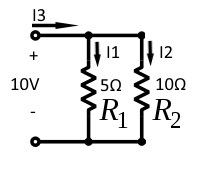
\includegraphics[scale=0.75]{parallelresistorsexample.png}
\label{fig:parallelresistorsexample}
\caption{Parallel Resistors Example}
\end{minipage}%
\begin{minipage}{.5\textwidth}
\centering
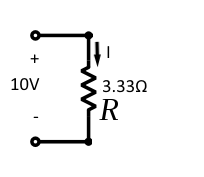
\includegraphics[scale=0.75]{parallelresistorsexamplemerged.png}
\label{fig:parallelresistorsexamplemerged}
\caption{Parallel Resistors Example Reduced}
\end{minipage}
\end{figure}

There are a few things to think about in this example. First, note that I3 in Figure \ref{fig:parallelresistorsexample} must be equivalent to the current I in Figure \ref{fig:parallelresistorsexamplemerged} since they are in truth the same circuit. In Figure\ref{fig:parallelresistorsexamplemerged}, we can easily solve for I using Ohm's law.

\begin{equation} \label{eqn:solvefori}
\begin{split}
V = IR \\
10 = I(3.33)\\
I = 10/3.33 \\
I = 3A
\end{split}
\end{equation}


We can likewise solve for I1 and I2 in Figure \ref{fig:parallelresistorsexample} using the same manner, but with R values of 5$\Omega$ and 10$\Omega$ respectively. This gives us I1 = 2A and I2 = 1A. Notice that I3 = I1 + I2. Another side-effect of Ohm's law is that the sum of all currents entering and leaving a node is 0, which is intuitive if you think about it. It's the same thing as splitting a hose. The sum of the volumes of water that come out of the two hoses must be the same as the volume that goes in to the un-split end.

\subsection{Blinking Lights}

One of the first things most people want to do with circuits is make lights blink. This is good. In the micro-controller world, you often don't have a terminal output until after you get through a decent amount of setup, so blinking LEDs can be the only way to debug problems during boot. The first thing most people do when they want to blink a light is blow one up. This should generally be avoided, although LEDs are cheap and it's a good learning experience.

First, let's look at the proper way to hook up an LED, shown in Figure \ref{fig:ledcircuit}. The main thing to note here is the resistor. Supplying too much current to an LED lets out the magic smoke, and remember, if you let out the magic smoke, the component no longer works. The next question, is how do you choose a value for R? This depends on the LED, and the voltage source. For kicks, let's assume you've got a 5V power supply, from an arduino GPIO for example. By the way, drawing too much power from an arduino GPIO is a good way to kill it, although the LED usually goes first. I'll assume you've got an LED that wants 10mA of current, although this may vary. Check the datasheet for your specific part.

There is one caveat about LEDs. We haven't talked about diodes because it's out of the scope of this document. However, LEDs are a special type of component called a "semi-conductor" which means it is only conductive some of the time. In this case, the LED is only conductive when it has at least a certain threshold of voltage pushing in the "correct" direction. Pay attention to which side the Anode and Cathode of your LED are plugged in to. If it's in the wrong way, current will not flow. (Unless you supply enough voltage to cause the diode to enter the "breakdown" voltage region. In this case, that's the amount of voltage where the LED breaks, but the breakdown region is actually very important for some components. Google "Zener Diode" for more on that. Hint: They're used in motor driver boards for back-emf protection.)

So why do we care about the LED being a semi-conductor? Because semi-conductors usually have a property called a "voltage-drop". This property causes the component to eat a portion of the voltage in the circuit. Your LED datasheet should say something about the voltage drop of the LED, but a typical value is 0.7V for hobby level LEDs. We typically model this voltage drop as a small voltage source pointed in the "wrong" direction. See Figure \ref{fig:ledcircuitvoltagedrop}.

\begin{figure}[h]
\centering
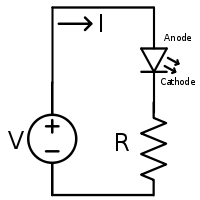
\includegraphics[scale=0.75]{ledcircuit.png}
\label{fig:ledcircuit}
\caption{LED Proper Hookup}
\end{figure}

\begin{figure}[h]
\centering
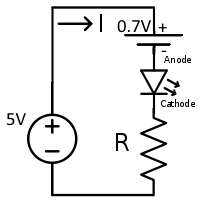
\includegraphics[scale=0.75]{ledcircuitvoltagedrop.png}
\label{fig:ledcircuitvoltagedrop}
\caption{LED Proper Hookup - With Voltage Drop}
\end{figure}

In this case we can just sum the two voltage sources, and pretend we have a 4.3V power supply. So, we have a 4.3V source, and we want a 10mA current. Easy, right? Just use Ohm's law as shown in Equation \ref{eqn:solveforr}.

\begin{equation} \label{eqn:solveforr}
\begin{split}
V = IR \\
4.3 = (.01)R\\
R = 4.3/.01 \\
R = 430\Omega
\end{split}
\end{equation}

It so happens that LEDs are generally pretty robust. You can probably go plus or minus about 50\% on that R value. A smaller value with make the LED brighter, while a larger value will make it dimmer. Too large a value will burn it out. An excessively large value \textit{may} make it explode. I highly recommend trying it once under controlled circumstances. Wear eye protection! There will probably be exactly one or two pieces of shrapnel, but it would really suck to get one in your eye. For best results, connect the LED to a power supply and slowly turn up the voltage. You'll get to see all phases of operation for the LED. Below 0.7V it probably will not turn on. From 0.7 to somewhere around 4-6V it will steadily get brighter. At some point it will reach a maximum brightness and then begin to heat up, at which point it will probably start to dim. At some point after that, it will go out. Cranking up the voltage more will (probably) cause it to explode. Sometimes the conductive element inside just melts and you don't get an explosion. It really depends on the LED.

\subsection{Voltage Divider}

There's one last circuit I want to mention because it becomes very important when dealing with analog sensors. The voltage divider. An example is shown in Figure \ref{fig:voltagedivider}. The basic idea here is that you have a known resistor value for R1, and some variable value for R2. A common one is a thermistor - a resistor that changes its value based on temperature. In fact, an excellent experiment to try is to use a thermistor in exactly this circuit configuration to measure the temperature of water. It's very easy, and will teach you about the analog to digital converter. There's also the matter of sensor calibration, but I won't go in to the details on that here. Suffice it to say that all sensors are terrible, and you should never trust them until you've tested them rigorously.

\begin{figure}[h]
\centering
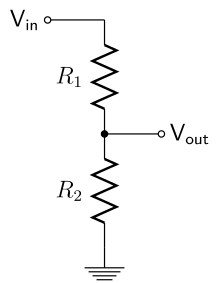
\includegraphics[scale=0.75]{voltagedivider.png}
\label{fig:voltagedivider}
\caption{Differential Drive}
\end{figure}

The general plan is to supply a known voltage to $V_{in}$, have a known $R_1$, and measure $V_{out}$. With these pieces of information, you can solve for $R_2$ using Ohm's law. The derivation isn't difficult, but other people have already done it, so here it is. Once you have $R_2$ you just refer to your sensor calibration or the datasheet for the part, and you have your value for (in this case) temperature.

\begin{equation} \label{eqn:solveforr}
\begin{split}
R_2 = R_1*\frac{1}{(\frac{V_{in}}{V_{out}}-1)}
\end{split}
\end{equation}

\section{Batteries}
\label{sec:batteries}

\subsection{The Basics}

We have had a lot of problems dealing with batteries over the years. Partly because people are lazy, but mostly because they don't understand how batteries work or how to properly maintain them. All batteries are basically slow, controlled, chemical reactions. They are not magical devices that store and dispense electric charge. The closest thing to that is a capacitor, which is two metal plates with an insulator between them. By applying voltage, you charged the plates, storing energy in the form of actual electric charge. However, capacitors tend to discharge all of their stored energy at once. In adddition, the total energy they can store is far less than most batteries. Batteries, on the other hand, store energy in the form of chemical potential energy. This is far more stable than storing raw electric charge, but it does lead to a few problems. The big on is that, since the energy storage relies on chemistry, temperature is important. Being stored in a place that is too hot or too cold can cause a battery to burst, or drain it. Another is that, over time, the chemistry can get disrupted, causing the battery's maximum storage potential to decline.

\subsection{Which Numbers Are Important?}

Now you know what voltage, current, and resistance all mean, but how do you use them in practice? 

\subsubsection{Voltage - V}

We'll start with voltage because that's the easiest one to handle. You want to make sure the voltage your batteries produces matches the voltage rating for the things you want to power: motors, cpu, sensors, etc. However, there's another consideration to make. You almost never want your batteries directly connected to your sensitive electronics. You always want a regulator of some sort in between. Why? As you drain a battery, the voltage will fluctuate. This can cause damage to unshielded electronics. We'll talk about regulators in Section \ref{sec:regulators}. In addition to the power fluctuations, you rarely have motors that you want to drive with the same voltage as the computer. In practice, you'll want to match your main battery voltage to the voltage of the motors you want to power, and then use regulators to smooth and reduce the voltage for the other components.

\subsubsection{Capacity - mAh}

This is the best measure of how much actual energy the battery can hold. To put it simply, a 1000mAh battery could sustain a drain of 1A for 1 hour before being depleted. If you draw 2A it will only last half an hour. At 0.5A, two hours. It's a very silly unit when you think about it, but it makes the math easy.

\subsubsection{C}

Most batteries have a C rating. This is a somewhat cryptic value that tells you how quickly a battery can discharge without damaging itself. This is not a limit on how much current the battery can draw. Remember Ohm's law? You thought it wasn't important, didn't you? The thing is, Ohm's law will dictate the current that gets drawn from the battery. The C rating just tells you what is safe. The tricky bit is that the actual safe rate of discharge depends on the size of the battery. Weird right? Here's the simple way to think about it. The amount of continuous current drain a battery can handle without damaging itself is obtained by multiplying the C rating with the battery capacity. For instance, a 1500mAh battery with a 5C rating can handle a continuous drain of 30,000mA or 30A.


\subsection{Lead Acid Batteries - Pb}

Lead acid batteries are very stable. That's why we use them in cars. They also have a pretty good capacity, and are able to source a tremendous amount of current at once. This is good, because it takes a lot of force to turn over an engine. For a rugged, outdoor robot that may experience a variety of temperature conditions, lead-acid may be the way to go. However, lead-acid batteries are generally larger and heavier than their counterparts. Charging them is easy. Just hook them up to a power supply, set the power supply to the battery's rated voltage, and limit the current. What you limit the current to depends on the battery. Car batteries can generally handle up to 6A. The real problem is heat. If you charge too fast, the metal plates in the battery heat up, and can cause the acid to boil. This creates potentially toxic vapors and, if the vapors escape the battery housing, reduce the lifespan and charge of the battery. Other than charging to quickly, there isn't much to worry about here. Please charge in a well-ventilated area, just in case. Running a lead-acid battery dead isn't really a big deal as long as you don't leave it dead for a long time, or it doesn't get to cold while dead.

\subsection{Lithium Polymer - LiPo}

In the robots I built during my time on the team, we used these most commonly. They are light-weight, small, and can store a great deal of power. A LiPo battery generally consists of some number of cells. Each cell has a rated voltage of 3.7V. Batteries with more voltage are built by putting multiple cells in series. This voltage has to do with the internal chemistry. LiPo batteries are not nearly as stable as lead acid. There are three major concerns when dealing with a LiPo. First, only charge using a LiPo charger. There are some extra pins on a LiPo battery that tell the charger important information about the cells within. Second, make sure you look up the rating for charging a LiPo. The general rule of thumb is that a LiPo can be charged at the rate of 1C. If you have a 1500 mAh battery, you can charge it at 1.5A. Charging it slower is fine. Charging faster can cause the LiPo to heat up, swell, and potentially burst. When the LiPo bursts, the chemicals inside will spontaneously burn, creating fire, pressure, and heat. Seriously bad news. Third, never ever cut or puncture a LiPo. An externally ruptured LiPo is bad news, but one that ruptures internally, or without a good pressure relief, is a thermal grenade.

That all said, LiPo batteries are pretty safe if you follow the guidelines I set out for charging. There are two more things to worry about. 3.7V is the rated voltage for a cell, but when you charge, you generally charge to about 4.2V - the charger will handle this. Never manually overcharge the LiPo. However, unlike a lead-acid battery, letting the charge get too low in a LiPo will permanently damage it. The minimum safe level for a single cell is 3V. Always monitor the voltage of LiPo batteries you are using and ensure they don't drop below this level. The difficult part is, LiPo voltage doesn't drop linearly. Figure \ref{fig:lipovoltage} shows voltage versus charge for a LiPo. As you can see from the graph, you have to monitor the battery voltage very carefully, because it decreases rapidly once the charge gets low.

\begin{figure}[h]
\centering
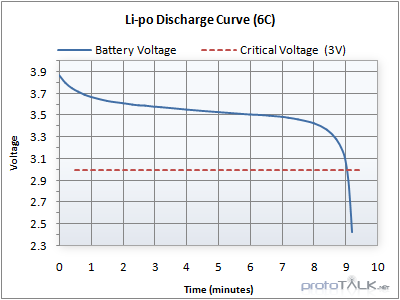
\includegraphics[scale=0.75]{lipovoltage.png}
\label{fig:lipovoltage}
\caption{LiPo Voltage VS Charge}
\end{figure}

As a side note, this chart is for one specific battery I found on a forum post at Traxxas.com. Individual results may vary in specifics, but the point is the same. Monitor your voltage and don't let it drop below 3.0V per cell. There is one additional caveat. LiPo batteries don't hold their charge forever, and they will, if left sitting on a shelf for long periods of time, eventually degrade. It is recommended to discharge and charge a LiPo battery every few months when it is not in active use. Discharging can be done by using the LiPo while closely monitoring the voltage, or with a dedicated charger. The chargers in the lab have this capability.

The final thing to mention is balancing. Because a LiPo battery may be made up of multiple cells, the total voltage isn't enough to tell the health of the battery. In the lab we have at least two balances. Some chargers will also balance while they charge. Balancing slowly bleeds charge from one cell and puts it into another cell. This keeps the cells from becoming unbalanced. This is a good thing. Each cell may discharge differently because chemistry is a sloppy science and never works quite the way it's supposed to. This can lead to one cell with a much higher or lower voltage than the others. If one cell gets overcharged, it may swell and/or rupture. If one cell gets too low, it may "die". Dead cells are ones that have dropped to a low enough voltage that they cannot safely be recharged. Most chargers will refused to charge the battery if there are dead cells. If you know what you're doing, sometimes dead cells can be nursed back to life, but it's a delicate and potentially dangerous procedure. It's usually better to recycle the battery and get a new one.

\subsection{Other Batteries}

There are three more common types of batteries. Lithium Iron Phosphate - LiFePO4 often pronounced "LieFo" - Nickle Metal Hydride - NiMH - and Nickle Cadmium - NiCd "Nigh-Cad". I haven't personally worked with either, so the internet is a better resource then I am. My vague understanding is that LiFePO4 are similar to LiPo batteries but more stable and more expensive. A quick Google search tells me that NiMH is the new NiCd, and is used in general consumer electronics, so it must be pretty stable, but doesn't (in general) have as much energy density as Lithium batteries.

\section{Tips For Not Lighting Things On Fire}

Forethought and attentiveness are key for keeping the magic smoke inside the components. All electrical components are made using plastic, silicon, some trace metals, and a mystical substance called magic smoke. If you give the component too much voltage, current, or heat the magic smoke will use this extra energy to break free and escape. It is a very clever substance, and even just a momentary spike is enough to free it. At this point the component will no longer work. Nobody is perfect, but here are a few tips I've picked up over the years to keep the magic smoke locked up tight.

\subsubsection{Turn Off The Power}

This should be common sense, but you'd be surprised how often people get overconfident about what they're doing and modify a circuit while it's powered. Sure, if you know what you're doing you're theoretically safe. The real problem arises when one of those tiny wires gets away from you. Powered wires appear to be supernaturally attracted to conductive terminals, particularly ones that will causes sparks. Just don't do it. The five seconds it takes to flip off the power could save you three days of waiting for new parts.

\subsubsection{Electrical Tape}

If you're working on a circuit, if you aren't immediately dealing with a wire, tape the end. Most of the instances in which I blew something up were because I forgot about a wire that wasn't connected, and it brushed up against something else, making a short. This is particularly important when dealing with batteries. Remember, you can't turn a battery off. If both terminals of a battery aren't connected to something, the free wires should be taped over.

Fun Fact: If you plug the gate pin on a MOSFET in to 24VDC, while the source is floating and the drain is grounded, it explodes.

\subsubsection{Be Careful Around Batteries}

I've alluded to this several times, but I'll say it again. Always be careful around batteries. I had six years of robotics team experience, and four years of that was while taking courses in Electrical Engineering. At the end of my last semester, I was putting different connectors on some LiPo batteries. I thought to myself, "I'll just cut both wires on the battery at the same time so they'll be the same length."

Technically speaking, it worked out. Turns out the reflex when you hear a loud SNAP and see a bright flash of light is to close your fist, which for me finished cutting the wires and yanked the tool away from the battery cables. It could have been worse though. Just think about what you're doing around batteries. Remember, they can't be turned off.

\subsubsection{Don't Work When You're Tired}

Or drunk. Or sick. Or angry. It makes you inattentive, and then things like the above happen. It doesn't matter how smart you are. Tired people make mistakes.

\subsubsection{Ground Loops}

Ground loops are tricky devils. Explaining the whole mechanism behind them is outside the scope of this document, however, if you are ever dealing with a circuit with multiple power sources, look them up. A ground loop can ruin your whole day. Essentially, ground loops occur when two things you consider "ground" have some resistance between them. If that happens, current through one loop induces a voltage difference in the other loop. Wikipedia is your friend here. Moral of the story - use isolated power supplies, and be very careful when plugging multiple power sources in to one set of electronics. When in doubt, unplug your computer from the wall before plugging anything grounded into it. USB cables, for instance.

\subsubsection{Use the Mult-Meter}

The multi-meter is your friend. When powering up a system for the first time, unplug all sensitive electronics, power the system, and check voltages at your main terminals. Make sure the value \textit{and} the polarity are correct. Then power down, plug in just one piece of equipment, and power back up. Repeat until everything is plugged in. This is useful for two reasons. First, if you have a problem, it will be very obvious which piece is the culprit. Second, if something blows, you risk damaging the minimum possible number of expensive items.

% !TEX root = HowToRobot.tex

\chapter{Odroid Setup}
\label{chap:odroidsetup}

\section{Purpose Of This Chapter}

This chapter is intended to be a guide for setting up an Odroid XU3 with Fedora 21, using an EMMC as the storage device. Step by step guides for using an SD card exist in plenty on the internet, and only the first two steps are any different. The steps should work with Fedora 22 as well, but Fedora 22 was still very new when I last worked with the Odroids and wasn't ready for installation on an arm architecture yet. For installation on other Odroid platforms, the steps should be very similar, but may not be exactly the same.

\section{Before You Begin}

You will need the following items to complete this guide:
\begin{enumerate}
\item{Odroid XU3}
\item{USB to MicroSD Adapter}
\item{MicroSD to EMMC Adapter}
\item{EMMC}
\item{Computer Running Fedora 20/21}
\item{USB to Serial Adapter}
\end{enumerate}

Check your version of Fedora before beginning. You can do this using the command:
\begin{lstlisting}[language=bash]
  $ cat /etc/issue
\end{lstlisting}

You want to check if you're running Fedora 20 or Fedora 21+. This will be important later.

\section{Obtain the Fuser}

The Fuser is a utility written by Scott Logan to set up the EMMC in such a way that the Fedora image fits on the EMMC efficiently. It sets the "fuse" bit, which are sort of like software-writable settings on the EMMC. Modifying these bits manually is pretty difficult, which is why you'll want to use the Fuser to do it for you.

On Fedora 21+, run:
\begin{lstlisting}[language=bash]
  $ sudo yum install smd-odroid-release
  $ sudo yum install odroid-xu3-sd-fuser
\end{lstlisting}

These two commands download repository information for the smd-odroid-release repository - which Scott maintains - and then downloads and installs the fuser itself.

Of Fedora 20, the repository headers will not automatically download. You'll have to download the fuser more directly. Instead run:

\begin{lstlisting}[language=bash]
  $ sudo yum install http://csc.mcs.sdsmt.edu/smd-odroid/fedora/linux/21/x86_64/odroid-xu3-sd-fuser-0.2.0-1.fc21.noarch.rpm
\end{lstlisting}

\section{Run The Fuser}

If you run in to problems, there is a wiki page with instructions specifically for the fuser at \url{https://github.com/sdsmt-robotics-odroids/odroid-xu/wiki/Boot-Media-Fusing}.

Before inserting the EMMC, run the command:

\begin{lstlisting}[language=bash]
  $ ls /dev/mmcblk*
\end{lstlisting}

Take note of the entries there. Whatever you see there before inserting the EMMC is what you will NOT want to target in the next steps. Next, connect the EMMC to your computer. Plug the EMMC into the EMMC to MicroSD adapter. If your machine has a MicroSD slot, you can plug that directly in to your computer. If not, (or if you encounter problems, which can happen rarely mostly due to driver issues) you'll need a MicroSD to USB adapter.

Run the ls command again. There should be new entries, probably something like /dev/mmcblkX... in a few various forms. Take note of the value of X. Now run the following command, substituting your number (usually 0) for X.

\begin{lstlisting}[language=bash]
  $ sudo odroid-xu3-emmc-fuser /dev/mmcblkX
\end{lstlisting}

You should see the following:
\begin{lstlisting}[language=bash]
    Successfully enabled write access to /dev/mmcblk0boot0.
	Fusing boot blob to /dev/mmcblk0boot0...
	1262+0 records in
	1262+0 records out
	646144 bytes (646 kB) copied, 1.71663 s, 376 kB/s
	Success!
\end{lstlisting}

If you don't see something like this, specifically if there are 0+0 records in or out, something has gone wrong. Try again or check the wiki instructions for the Fuser.

\section{Loading The EMMC Image}

First you need to get the image to write to the EMMC. The images are hosted at \url{http://csc.mcs.sdsmt.edu/smd-odroid/fedora/linux/21/Images/armhfp/}. You'll want to download the "latest" image for your type of Odroid. In this case, the filename will probably be something like: f21-odroid-xu3-minimal-latest.img.xz.

Once you have downloaded the image, uncompress it using the following command with <foo> replaced by the image name. This will take about a minute.

\begin{lstlisting}[language=bash]
  $ xz -d <foo>.img.xz
\end{lstlisting}

Next, you need to unmout the EMMC partitions or they won't write correctly. Do so with the following command, again substituting your value for X:

\begin{lstlisting}[language=bash]
  $ sudo umount /dev/mmcblkXp*
\end{lstlisting}

Be careful with this next command. dd is a very powerful tool, and it can totally erase your harddrive if you let it. Mostly just make sure you don't accidentally point it at the wrong device. if is the input file - the image you uncompressed. of is the target device, the mmblkX we identified earlier. Substitute your value for X. bs is the block size. Just leave it alone.

\begin{lstlisting}[language=bash]
  $ sudo dd if=<foo>.img of=/dev/mmcblkX bs=8M
\end{lstlisting}

This takes a while. On the order of 3 or 4 minutes when I did it last. Be patient. When it finishes, you should expect to see:
\begin{lstlisting}[language=bash]
    204+1 records in
	204+1 records out
	1713373184 bytes (1.7 GB) copied, 91.7598 s, 18.7 MB/s
\end{lstlisting}

Next, to make sure the OS has flushed all the buffers to the device, run:

\begin{lstlisting}[language=bash]
  $ sync
\end{lstlisting}

If there is a noticeable pause after running sync, run it again just in case. That pause means it's working on something. If there is no noticeable pause, it didn't do anything, and you're good to go.

\section{What Next?}

At this point, you have a functional EMMC with Fedora 21 installed. Go ahead and plug it back in to the Odroid. I recommend getting a USB-Serial converter cable to debug with. I also recommend getting a CMOS battery for the Odroid, or the system clock will reset every time the board is restarted. This makes yum unhappy and you'll have a bad time. ROS can throw some very strange time-related errors as well. If you only needed Fedora installed, you're done with this chapter - except perhaps see the section on common error messages. Otherwise, move on to the next section to install ROS. It's possible the Scott has the kick-start version up by now, with ROS already installed, but at the time of writing, that hasn't happened yet.

\section{Installing ROS}

The ROS build for arm isn't in with the normal ROS or Linux repositories. It was in fact hosted from, when I left, a set of 10 Odroids over in M113. To install this repository, run:

\begin{lstlisting}[language=bash]
  $ sudo yum install http://csc.mcs.sdsmt.edu/smd-pub/fedora/linux/21/armhfp/smd-ros-release-21-2.noarch.rpm
\end{lstlisting}

You'll also need rpm fusion, which is an extended set of packages for Fedora not bundled in to the main set of rpms. To install those, run:

\begin{lstlisting}[language=bash]
  $ sudo yum localinstall --nogpgcheck http://download1.rpmfusion.org/free/fedora/rpmfusion-free-release-$(rpm  -E %fedora).noarch.rpm http://download1.rpmfusion.org/nonfree/fedora/rpmfusion-nonfree-release-$(rpm -E %fedora).noarch.rpm	
\end{lstlisting}

Now, you should be able to use yum to install pretty much any ROS Fedora package. The following command will install the basic starting ROS packages. It doesn't not include PCL or Gazebo, but you shouldn't be running those on Odroids anyway.

\begin{lstlisting}[language=bash]
  $ sudo yum install ros-indigo-robot	
\end{lstlisting}

If you want to do on-board compiling, which you almost certainly will unless you've already finished development and are just deploying functional binaries, run the following command:

\begin{lstlisting}[language=bash]
  $ sudo yum install python-rosdep python-rosinstall_generator python-wstool python-rosinstall @buildsys-build	
\end{lstlisting}

That's it. Installing ROS is way easier than it used to be. If in doubt, here's a link to the ROS wiki page dealing with installation issues: \url{http://wiki.ros.org/indigo/Installation/Source}.

This is a fairly basic install, so there may be some unresolved dependencies. If you're having dependency issues, run the following command where <src> is a directory containing ROS packages.

\begin{lstlisting}[language=bash]
  $ rosdep install --from-path <src> --ignore-src	
\end{lstlisting}

\section{Common Errors}

There are a handful of pretty common errors that I found solutions for:

\begin{lstlisting}[language=bash]
  One of the configured repositories failed (Fedora 21 - x86_64 - Updates),
and yum doesn't have enough cached data to continue. At this point the only
safe thing yum can do is fail. There are a few ways to work "fix" this:

 1. Contact the upstream for the repository and get them to fix the problem.

 2. Reconfigure the baseurl/etc. for the repository, to point to a working
    upstream. This is most often useful if you are using a newer
    distribution release than is supported by the repository (and the
    packages for the previous distribution release still work).

 3. Disable the repository, so yum won't use it by default. Yum will then
    just ignore the repository until you permanently enable it again or use
    --enablerepo for temporary usage:

        yum-config-manager --disable updates

 4. Configure the failing repository to be skipped, if it is unavailable.
    Note that yum will try to contact the repo. when it runs most commands,
    so will have to try and fail each time (and thus. yum will be be much
    slower). If it is a very temporary problem though, this is often a nice
    compromise:

        yum-config-manager --save --setopt=updates.skip_if_unavailable=true

Cannot retrieve metalink for repository: updates/21/x86_64. Please verify its path and try again.	
\end{lstlisting}

So this is a pretty scary error, but the actual cause is pretty tame. This happens once on almost every new Odroid install. The root cause is actually that the internal clock is set way back in the past to a time where the repository didn't exist. So when yum tries to check for the repository certificates, none of them are valid yet. To verify that this was the problem use the command:

\begin{lstlisting}[language=bash]
  $ date
\end{lstlisting}

If your Odroid is kickin' it in the '70s. You've found the problem. This is an easy fix. Run the following commands. The first updates the current time using the ntp server on campus. The second updates the hardware clock, which persists between power cycles provided you have that CMOS battery installed. If not, you'll have to do this every time.

\begin{lstlisting}[language=bash]
  $ ntpdate ntp.sdsmt.edu
  $	hwclock -w
\end{lstlisting}

There was, last time I spoke to Scott, a potential problem with a dtb file not being updated in the kernel. If this happens and causes problems, just get a new image and repeat this process. Scott was hoping to have this fixed soon, so it's probably already done by now, but I'll leave this warning here anyway.
%% !TEX root = Proposal.tex

\chapter{Implementation}
%% !TEX root = Proposal.tex

\chapter{Evolving Behavior}
\label{chap:ann}

\section{Structure}
The Critters use an Artificial Neural Network (ANN) to determine their behavior. To put it academically, the ANN is a single layer feed forward perceptron net which uses a sigmoid activation that has been stretched and shifted to allow values between -1 and 1. To put it more simply, each Critter has a tiny brain with a series of input cells and output cells. The input cells include 4 static cells which tell the Critter about its current health and life points. There are also 2 input cells for each eye, which tell the critter whether or not the eye detects an enemy, and whether or not the eye detects food. There are three outputs which tell the Critter to move forward or backward, left or right, or to turn left or right. To reiterate, the structure of the ANN for each Critter was not static, and the number of input nodes varies with the number of eyes.

\section{Crossover}
Crossover with a non-static ANN was tricky. Different parents could have different numbers of eyes, which meant we couldn't just average values from the parents' ANNs to create a child. To get around this, each Eye had its own miniature ANN with 3 outputs, and to get the output for the whole ANN, we just took the sum of the results from all of the eyes and the four static input nodes. This way eyes could be dropped or added from the network without changing the rest of the net.

When preforming crossover, the child has a chance to inherit eyes from the parents. If both parents have 1 eye, the child has a 45\% chance to inherit each parent's Eye, including the ANN. There is also a 10\% chance to not inherit an eye. This continues for each Eye that both parents possess. For example, if one parent has 2 eyes, and one has 3, the child has a 45\% chance to inherit from parent 1 or 2 for the first 2 eyes. For the third eye, the child has a 50\% chance to inherit from the parent with 3 eyes, and a 50\% chance to inherit no eye.

\section{Mutation}
In contrast with Crossover, mutation for the eyes and the Neural Net The characteristics for each eye, and the weights in the ANN for each Eye are mutated using the guidelines in Chapter\autoref{chap:reproduction}. 
%% !TEX root = Proposal.tex

\chapter{Evolution}
\label{chap:reproduction}

Like many evolutionary systems, the critters evolve through reproduction and mutation so their species lives on. To determine who is resurrected and who is replaced for the next round, the critters are ranked. Their rank is determined by how long they lived. Theoretically, the longer they live, the better suited to the environment they are and so, their ranking is higher. Anti-vaccers have disproven this theory but we're going to roll with it. After the ranking, the top 50\% of the population is kept for the next round and used as Parents for the crossover mutation, discussed later. The bottom 50\% is replaced with the 'children' of the top 50\%. \\
\newline
It should be noted that all non-eye characteristics such as attack, defense, etc. are handled in one reproductive function and all eye characteristics such as number, field of view, etc. are handled in a different function. This is because all non-eye characteristics are handled as doubles and the number of them do not change, while the eye characteristics involve dynamic memory due to the variation of the number of eyes. \\
\newline
To simulate a real critter reproducing, the crossover and mutation genetic algorithms were used to create the next generation of critters. Each were applied in two different ways to handle the non-eye characteristics and eye characteristics. 

\section{Crossover}
The crossover method, takes two parents, picks a random spot to cut their 'DNA' and splices the first chunk from Parent A to the second chunk from Parent B. This method works well for the non-eye characteristics, which are held in an indexable array. A random number in the array index range is chosen as the 'cut point'. Then the characteristics before that index are copied from Parent A and the characteristics after and including the index are copied from Parent B. \\

For the eyes, handling crossover is much trickier. To imitate real life, the child would have a chance at inheriting either Parent A's eye, Parent B's eye or no eye at all for the minimum number of eyes present. Then, the child would have a chance of inheriting or not inheriting the eye from the parent with more eyes. For example, if Parent A had two eyes and Parent B had three eyes, for the first two eyes, the characteristics would come from Parent A or Parent B. For the third eye, the child would either inherit the eye from Parent B or no eye at all. 


\section{Mutation}
The mutation method simply perturbs the current values by small amounts. In the configuration file, there are two user definable parameters for mutation: Mutation Rate and Mutation Chance. The Mutation Rate is how much a parameter can mutate. The Mutation Chance is the chance a characteristic will mutate. For the non-eye characteristics, a random number is generated for each characteristic and if that beats the Mutation chance, it is mutated. It's mutated with equation ~\ref{mutate-eqn}, where percent is a value between -1 and 1. 

\begin{equation}
val_{new} = val_{old} + (percent) (mutation_{rate})
\end{equation} \label{mutate-eqn}


The eyes are once again, a special case. They are mutated in two loops. First, the number of eyes is given a chance to mutate, which is user defined in the configuration file. The critter can either loose an eye or gain an eye. Then, the characteristics associated with the eye are mutated using the same methodology as the non-eye characteristics. 






%% !TEX root = Proposal.tex

\chapter{Project Results}
\label{chap:results}

\section{Initial Conditions}

One thing that we noticed (and expected) is that the long-term behavior of the simulation is very sensitive to the game configuration parameters. For example, in our early simulations we discovered that the metabolic cost of eyes compared to the benefit of having the eyes would often lead to eyes being abandoned altogether in the first handful of generations.

\section{Eyes}

Of the two major aspects of this project, evolving behaviors was perhaps the more interesting. Unfortunately, we didn't see interesting behaviors emerging as regularly or as quickly as we hoped. We attribute this to two main factors.

First, eyes are expensive, but also required for complex behavior. This is somewhat realistic, but leads to being trapped in a local maxima with no eyes. Evolving good behaviors seems to take longer than just evolving the eyes away, so most simulations end up reducing to the minimum allowable number of eyes. We theorize that if we were to allow mutation and crossover on the Neural Nets with greater frequency than the characteristics, the Critters might be forced to evolve behaviors rather than just reducing metabolic cost by dropping eyes.

Second, the Critters are stupid. The ANN we used for behavior is very simple and has no concept of memory or context. We theorize that with a more complex Neural Net, more complex behaviors could emerge.

Although the eyes weren't always used effectively, some behavior that did somewhat commonly emerge was very nimbly avoiding other Critters (and sometimes food).

\section{Populations}

One of our original goals was to demonstrate stratification among different populations in the same environment. In other words, we wanted to create a situation in which there wasn't one "correct" genome. Rather, we wanted an environment in which the "best" configuration for each population depended on the current configuration of the other populations. We didn't see as much of this as we hoped.

We didn't see this as much as we had hoped, although it did happen on occasion. This is in large part because the Critters commonly all reduce to low metabolic cost states, which tend to be small Critters with the minimum number of eyes.

\section{Motion}
A popular method for many critters, particularly those with no eyes, was to spin in tight circles. We theorize this is because it would minimize chances of combat. Critters with eyes were also able to more completely observe their immediate surroundings. Occasionally a critter would evolve to have a lot speed and to travel a wide circle. This made them likely to ram into others, killing them and gaining life. These Critters also had more success at randomly eating food because they covered more ground. 

\section{Aggression}
We tried really hard to set up a configuration that would lead to a predatory population. However, this requires characteristics and behaviors to evolve together. In addition, since Critters don't know anything about the Critters they're observing, they have no idea if the target is weaker or stronger than they are. It was almost always safer to just avoid confrontation, even if it meant they didn't get the rather large life and health bonus for scoring a kill. Adding some more information about the enemy sighted to the neural net would likely allow the Critters to evolve more complex predatory behaviors.


%%! TEX root = Proposal.tex

\chapter{Future Work}
\label{futureWork}

There are many interesting paths this project can take, such as:

\begin{itemize}[noitemsep]
	\item Exploratory Motion for Critters with Eyes
	\item Weighted Eye Crossover
	\item Toroidal Environment
	\item 3D Environment
	\item Environment Conditions
	\item Complex Food Sources
	\item Obstacles 
	\item Subranking
\end{itemize} 

\section{Exploratory Motion}
In the simulations run, many of the critters would spin in place or in a small circle, much like young ballerinas. This doesn't really make sense for critters with eyes. Introducing some sort of rudimentary motion control to kickstart the ANN for critters with eyes might produce more interesting results, prevent the eyes from dying off so quickly and force them to evolve motion in a more intelligent manner. Perhaps they could start off with a Brownian Walk and evolve into smooth curves. 

\section{Crossover}
A modification to the crossover eye method could speed convergence or find a local extrema.  The chance to inherit an eye would be weighted in favor of the higher ranked parent.  \\

\section{Toroidal Environment}
An Asteroid's like toroidal environment would prevent the critters from getting stuck in the corners. Another affect would be to allow the prey in a predator-prey relationship to run away without trapping themselves into an 'unseen' corner.\\

\section{3D Environment} 
A three dimensional environment would significantly increase the math done behind the scene. It's an easy extension but significant amounts of code would need to be re-written for collision, motion, the ANN, eyes, drawing, etc.\\

\section{Environment Conditions}
To simulate real life, the environment could have properties and those properties could be changed over time. Properties could be temperature variations, visibility variations and water salinity. Temperature variations could cause populations to evolve in warmer or cooler areas and when a temperature flux is induced, they may die off or thrive. Visibility variations would have a direct impact on the cost of eyes. Creatures that can see well in poor visibility would have more energy allocated to eyes so they might move slower but become better at luring prey to them. Water salinity would have similar repercussions as temperature.\\


\section{Complex Food Sources}
More complex food source schema could have interesting impacts on the environment. One method is where the critter has a food conversion efficiency and the food source has a nutritional value. This would force the critter to increase their food conversion efficiency and to identify food sources with a better nutritional value. (A method that seems to have been lost on many CS students.) \\

\section{Obstacles}
Implementing obstacles would not be terribly difficult. There would be two types, benign and malicious. Benign obstacles would do no damage to a critter running into it but could also offer shelter to a prey critter. Offering shelter would definitely work better in a three dimensional environment and with a less simplistic model of physics. A malicious obstacle would injure the critter. If a predator-prey behavior emerges, perhaps the predators could develop a herd like mentality to run prey into the malicious obstacle to prevent damage to themselves. To implement these change, some underlying code structures would need to be changed in order need to identify the difference between benign and malicious. \\


\section{Subranking}
Currently, the critters are ranked solely on lifetime. Initially, many creatures die off due to the lifetime points running out but have taken some damage from blindly running into other creatures. Our sorting method may rank a critter that lived the entire time but died with one or two health points left over a critter that also lived the same amount of time but died at full health. Ideally, the one with full health would be ranked above the one with a few points left at the end. \\


%%%  Done with chapters
% Bib stuff

\bibliographystyle{IEEEtran}
\bibliography{refs.bib}
\input{refs.bib}
\addcontentsline{toc}{chapter}{Bibliography}


\appendix
%% !TEX root = Proposal.tex

\chapter{Original Proposal}
\label{chap:originalProposal}
\section{Abstract}

For our final project in Natural Computing, we plan on creating an artificial life simulation involving the evolution of characteristics and behaviors for simulated creatures. The project will feature a set of fixed physical characteristics and a neural network for each individual. Each of the characteristics, such as speed, size, health points, number of eyes, and combat skill, will have an associated metabolic cost. For instance, a large, powerful individual will require more food to survive than a smaller weaker creature, but be able to kill the weaker creature for food. The neural network associated with each individual will be used to determine the individual's behavior given sensory information. The topology for the neural net of each individual will vary based on the number of sensory organs the individual has. Only the input layer of the neural net will be subject to changes in topology. The rest of the net will be fixed. A tournament style ranking will be employed for selection, and both mutation and crossover will be applied to the characteristics and neural networks.

\section{Project}

The inspiration for this project comes from a video posted on YouTube by Paul Oliver dealing with an artificial life simulation \cite{oliver}. While the video was the initial inspiration for the project, we wanted to take the idea further than the original author did.

The traits of each creature will be the following:

\begin{itemize}[noitemsep]
  \item Number of eyes
  \begin{itemize}[noitemsep]
     \item Eye placement
     \item Eye view distance
     \item Eye view arc
  \end{itemize}
  \item Max Health
  \item Health Regen
  \item Size
  \item Attack Power
  \item Defense
  \item Speed
  \item Metabolic Cost
\end{itemize}

Most of the items listed are self explanatory, but a few deserve special attention. Each creature will have a metabolic cost associated with each of its physical characteristics. A faster creature, or a stronger creature, will incur a heavier metabolic cost and therefore require more food to survive. The number of eyes also deserves special note because it inherently changes the structure of the neural network used to determine the creature's behavior.
\\
\\
The program will be structured as a tournament based, generational, evolutionary model.

\section{Selection}

Selection of individuals for survival from generation to generation will be done by a strict ranking. The ranking will be determined by performance in a tournament. The entire population will be randomly placed in the simulated environment, and the simulation will be run until all individuals have starved. To prevent simulations from running forever, the amount of food released into the environment will be reduced based on the number of remaining individuals, and based on the amount of time that has passed. The amount of time that an individual survives in time-steps will be their fitness, with a higher fitness being desirable. The least fit individuals each generation will be removed, and their places filled by crossover to keep a constant population.

\section{Crossover}

Selection for crossover will be done roulette style based on the fitness of the parents. Thus an individual with a higher fitness has a higher chance of being selected as a parent. Crossover will be done in two ways. For the physical characteristics, the values for the characteristics will be averaged. Note that the metabolic cost is derived from the other characteristics and is not subject to change via mutation or crossover. When applicable, the neural net weights will also be averaged. However, because of the non-static nature of the neural nets, special steps are required to do crossover between two individuals with non-similar neural nets. The details of this crossover are yet to be determined, but we speculate that the weights in the input layer of the network will be associated with the input organ they originate from. If the new creature has fewer eyes than one of the parents, the weights from the extra eyes will be ignored, whereas eyes that exist in the child but not in either parent will have randomly generated weights. For eyes that existed in one parent but not the other, the weights will be copied from the parent with the eye. If both parents had the same number of eyes, the weights are simply averaged.

\section{Mutation}

Each generation, after Mutation will be done on each individual in two ways. For a selected individual, each physical characteristic will have a chance to undergo a mutation. The exact nature of each mutation will vary from parameter to parameter, but in general each characteristic will be modified by a percentage of the previous value. For the neural net, each weight in the net will have a small chance of being mutated in a similar fashion.

\section{Other Details}

The simulation will be visualized through OpenGL. In order to speed up run times to a bearable degree, the population sizes will be kept small, and only one in every N runs will be displayed to the user. The rest will be run without graphics. Depending on run-times for the background simulation, some basic statistics may be printed in a window so the program does not appear to have frozen.
%% !TEX root = Proposal.tex

\chapter{User's Guide}
\label{chap:user}

\section{Build Instructions}
This application was developed and does function on a Fedora 20 machine. Type "make", the executable will be named "ALifeFishTank", and run "ALifeFishTank". There is a configuration file where various parameters can be changed.

\section{Configuration File}
Changeable parameters are listed below:

\begin{itemize}[noitemsep]
	\item Num\_Population - Number of populations (species)
	\item Population\_Size - Number of individuals in the population
	\item Max\_Life\_Time - Starting life time for all individuals
	\item Min\_Eyes - Minimum number of eyes any individual may have
	\item Max\_Eyes - Maximum number of eyes any individual may have
	\item Eye\_Cost - Metabolic cost of having an eye
	\item Min\_Eye\_FOV - Minimum field of view for an eye
	\item Max\_Eye\_FOV - Maximum field of view for an eye
	\item FOV\_Cost - Metabolic cost for the field of view
	\item Min\_Eye\_Range - Minimum distance an eye can see
	\item Max\_Eye\_Range - Maximum distance an eye can see
	\item Range\_Cost - Metabolic cost for eye range
	\item Min\_Max\_Health - Minimum max health an individual may have
	\item Max\_Max\_Health - Maximum max health an individual may have
	\item Max\_Health\_Cost - Metabolic cost of having health
 	\item Min\_Size - Minimum size of the individual
	\item Max\_Size - Maximum size of the individual
	\item Size\_Cost - Metabolic cost of size
	\item Min\_Attack - Minimum attack
	\item Max\_Attack - Maximum attack
	\item Attack\_Cost - Metabolic cost of attack
	\item Min\_Defense - Minimum defense
	\item Max\_Defense - Maximum defense
	\item Defense\_Cost - Metabolic cost of defense
	\item Min\_Speed - Minimum move speed
	\item Max\_Speed - Maximum move speed
	\item Speed\_Cost - Metabolic cost of speed
	\item Global\_Mutation\_Rate - Mutation Rate if a population rate is not defined
	\item Global\_Mutation\_Chance - Mutation Chance if a population chance is not defined
	\item Pellet\_Initial\_Drop\_Rate - Start drop rate of food pellets
	\item Pellet\_Drop\_Decay\_Rate - Decay rate of pellet drop
	\item Food\_Pellet\_Health\_Bonus - Health bonus for eating a food pellet
	\item Kill\_Health\_Bonus - Health bonus for killing another critter
	\item Food\_Pellet\_Life\_Bonus - Life bonus for eating a food pellet
	\item Kill\_Life\_Bonus - Life bonus for killing another critter
	\item Mutation\_Rate - Mutation rate for a population
	\item Mutation\_Chance - Mutation chance for a population
\end{itemize}

%\chapter{Code}
%% ! TEX root = Proposal.tex

\section{Header Files}
\subsection{Critter.h}
\lstinputlisting{../include/Critter.h}

\newpage
\subsection{Eye.h}
\lstinputlisting{../include/Eye.h}

\newpage
\subsection{GameController.h}
\lstinputlisting{../include/GameController.h}

\newpage
\subsection{maindisplay.h}
\lstinputlisting{../include/main_display.h}

\newpage
\subsection{main.h}
\lstinputlisting{../include/main.h}

\newpage
\subsection{MutableParameters.h}
\lstinputlisting{../include/Mutable_Parameters.h}

\newpage
\subsection{Population.h}
\lstinputlisting{../include/Population.h}

\newpage
\subsection{SharedConstants.h}
\lstinputlisting{../include/SharedConstants.h}

\newpage
\subsection{Structs.h}
\lstinputlisting{../include/Structs.h}

\section{Source Files}
\lstinputlisting{../src/Critter.cpp}

\newpage
\subsection{Eye.cpp}
\lstinputlisting{../src/Eye.cpp}

\newpage
\subsection{GameController.cpp}
\lstinputlisting{../src/GameController.cpp}

\newpage
\subsection{Main.cpp}
\lstinputlisting{../src/main.cpp}

\newpage
\subsection{mainDisplay.cpp}
\lstinputlisting{../src/main_display.cpp}

\newpage
\subsection{MutableParameters.cpp}
\lstinputlisting{../src/MutableParameters.cpp}

\newpage
\subsection{Population.cpp}
\lstinputlisting{../src/Population.cpp}


%Images and source locations
%Differential Drive, Ackerman Drive, Skid Steer - http://www.robotplatform.com/knowledge/Classification_of_Robots/wheel_control_theory.html
%Mecanum Drive - 
% Voltage Divider Image - http://learning.codasign.com/index.php?title=File:Voltage_divider_schematic.png
% Other circuits: Wikipedia

\end{document}
